%% abtex2-modelo-trabalho-academico.tex, v-1.9.7 laurocesar
%% Copyright 2012-2018 by abnTeX2 group at http://www.abntex.net.br/ 
%%
%% This work may be distributed and/or modified under the
%% conditions of the LaTeX Project Public License, either version 1.3
%% of this license or (at your option) any later version.
%% The latest version of this license is in
%%   http://www.latex-project.org/lppl.txt
%% and version 1.3 or later is part of all distributions of LaTeX
%% version 2005/12/01 or later.
%%
%% This work has the LPPL maintenance status `maintained'.
%% 
%% The Current Maintainer of this work is the abnTeX2 team, led
%% by Lauro César Araujo. Further information are available on 
%% http://www.abntex.net.br/
%%
%% This work consists of the files abntex2-modelo-trabalho-academico.tex,
%% abntex2-modelo-include-comandos and abntex2-modelo-references.bib
%%

% ------------------------------------------------------------------------
% ------------------------------------------------------------------------
% abnTeX2: Modelo de Trabalho Academico (tese de doutorado, dissertacao de
% mestrado e trabalhos monograficos em geral) em conformidade com 
% ABNT NBR 14724:2011: Informacao e documentacao - Trabalhos academicos -
% Apresentacao
% ------------------------------------------------------------------------
% ------------------------------------------------------------------------

\documentclass[
	% -- opções da classe memoir --
	12pt,				 % tamanho da fonte
	oneside,			 % para impressão em recto.
	a4paper,			 % tamanho do papel.
	% -- opções da classe abntex2 --
	chapter=TITLE,		 % títulos de capítulos convertidos em letras maiúsculas
	section=TITLE,		 % títulos de seções convertidos em letras maiúsculas
	sumario=tradicional, % estilo do sumário (tradicional = indentado)
	% -- opções do pacote babel --
	english,			 % idioma adicional para hifenização
	french,				 % idioma adicional para hifenização
	spanish,			 % idioma adicional para hifenização
	brazil				 % o último idioma é o principal do documento
	]{abntex2}

% ---
% Pacotes básicos 
% ---
\usepackage{helvet}			    % Usa a fonte Helvet			
\usepackage[T1]{fontenc}		% Selecao de codigos de fonte.
\usepackage[utf8]{inputenc}		% Codificacao do documento (conversão automática dos acentos)
\usepackage{indentfirst}		% Indenta o primeiro parágrafo de cada seção.
\usepackage{color}				% Controle das cores
\usepackage{graphicx}			% Inclusão de gráficos
\usepackage{microtype} 			% Para melhorias de justificação
\usepackage{lib/unifacens}      % Adaptações as normas da UniFacens
\usepackage{pdfpages}           % Para incluir pdf no documento
\usepackage{ragged2e}           % Para alinhamento de texto
\usepackage{titlesec}
% ---
		
% ---
% Pacotes adicionais, usados apenas no âmbito do Modelo Canônico do abnteX2
% ---
\usepackage{lipsum}				% para geração de dummy text
% ---

% ---
% Pacotes de citações
% ---
\usepackage[brazilian,hyperpageref]{backref}	 % Paginas com as citações na bibl
\usepackage[alf]{abntex2cite}	% Citações padrão ABNT

% --- 
% CONFIGURAÇÕES DE PACOTES
% --- 

% ---
% Configurações do pacote backref
% Usado sem a opção hyperpageref de backref
\renewcommand{\backrefpagesname}{Citado na(s) página(s):~}
% Texto padrão antes do número das páginas
\renewcommand{\backref}{}
% Define os textos da citação
\renewcommand*{\backrefalt}[4]{
	\ifcase #1 %
		Nenhuma citação no texto.%
	\or
		Citado na página #2.%
	\else
		Citado #1 vezes nas páginas #2.%
	\fi}%
% ---

% --- 
% CONFIGURAÇÕES DE ESTILO E TAMANHO DA FONTE
% --- 

% Define a fonte padrão como serif (Arial)
\renewcommand{\familydefault}{\sfdefault}

% Define o tamanho da fonte dos capitulos para 14pt.
\renewcommand*{\chapnumfont}{\normalfont\large\bfseries\sffamily}
\renewcommand*{\chaptitlefont}{\normalfont\large\bfseries\sffamily}

% Define o tamanho da fonte das seções e sub-seções para 12pt,
% sendo as seções em negrito.
\setsecheadstyle{\normalsize\bfseries}
\setsubsecheadstyle{\normalsize}
% ---

\graphicspath{{./images/}}

% ---
% Informações sobre o trabalho
% ---
\coordenadoria{Coordenadoria de Engenharia da Computação}
\titulo{Titulo do trabalho}
\subtitulo{Subtitulo se houver}
\integranteum{Nome do aluno 1}
\integrantedois{Nome do aluno 2}
\local{Sorocaba/SP}
\data{2021}

% ---
% Informações sobre orientador
% ---
\orientador{Nome do orientador}

% ---
% Informações sobre coorientador
% ---
\coorientador{}

% O preambulo deve conter o tipo do trabalho, o objetivo, 
% o nome da instituição e a área de concentração 
\preambulo{Trabalho de conclusão de curso apresentado ao Centro Universitário Facens como exigência parcial para obtenção do diploma de graduação em Engenharia da Computação.\\ Orientador: Prof. ---------------------------}
% ---


% ---
% Configurações de aparência do PDF final

% alterando o aspecto da cor azul
\definecolor{blue}{RGB}{41,5,195}

% informações do PDF
\makeatletter
\hypersetup{
     	%pagebackref=true,
		pdftitle={\@title}, 
		pdfauthor={\@author},
    	pdfsubject={\imprimirpreambulo},
	    pdfcreator={LaTeX with abnTeX2},
		pdfkeywords={abnt}{latex}{abntex}{abntex2}{trabalho acadêmico}, 
		colorlinks=true,       		% false: boxed links; true: colored links
    	linkcolor=black,          	% color of internal links
    	citecolor=blue,        		% color of links to bibliography
    	filecolor=magenta,      		% color of file links
		urlcolor=blue,
		bookmarksdepth=4
}
\makeatother
% --- 

% ---
% Posiciona figuras e tabelas no topo da página quando adicionadas sozinhas
% em um página em branco. Ver https://github.com/abntex/abntex2/issues/170
\makeatletter
\setlength{\@fptop}{5pt} % Set distance from top of page to first float
\makeatother
% ---

% ---
% Possibilita criação de Quadros e Lista de quadros.
% Ver https://github.com/abntex/abntex2/issues/176
%
\newcommand{\quadroname}{Quadro}
\newcommand{\listofquadrosname}{Lista de quadros}

\newfloat[chapter]{quadro}{loq}{\quadroname}
\newlistof{listofquadros}{loq}{\listofquadrosname}
\newlistentry{quadro}{loq}{0}

% configurações para atender às regras da ABNT
\setfloatadjustment{quadro}{\centering}
\counterwithout{quadro}{chapter}
\renewcommand{\cftquadroname}{\quadroname\space} 
\renewcommand*{\cftquadroaftersnum}{\hfill--\hfill}

\setfloatlocations{quadro}{hbtp} % Ver https://github.com/abntex/abntex2/issues/176
% ---

% ---
% Adaptações para atender o sumário da biblioteca FACENS
%

% Define os capítulos como caixa alta
\makeatletter
\settocpreprocessor{chapter}{%
    \let\tempf@rtoc\f@rtoc% 
    \def\f@rtoc{%
      \texorpdfstring{\MakeTextUppercase{%
        \tempf@rtoc}%
      }{\tempf@rtoc}%
    }% 
}
\makeatother

% define seções como caixa alta
\makeatletter
\let\oldcontentsline\contentsline
\def\contentsline#1#2{%
  \expandafter\ifx\csname l@#1\endcsname\l@section
    \expandafter\@firstoftwo
  \else
    \expandafter\@secondoftwo
  \fi
  {%
    \oldcontentsline{#1}{\MakeTextUppercase{#2}}%
  }{%
    \oldcontentsline{#1}{#2}%
  }%
}
\makeatother

% define capítulo de referencias como caixa alta
\renewcommand{\bibsection}{%
    \chapter*{\bibname}
    \bibmark
    \ifnobibintoc\else
    \phantomsection
    \addcontentsline{toc}{chapter}{\uppercase{\bibname}}
    \fi
    \prebibhook
}

% remove identação
\cftsetindents{chapter}{0cm}{0.5cm}
\cftsetindents{section}{0cm}{0.8cm}
\cftsetindents{subsection}{0cm}{1.1cm}
% ---

% --- 
% Espaçamentos entre linhas e parágrafos 
% --- 

% O tamanho do parágrafo é dado por:
\setlength{\parindent}{1.3cm}

% Controle do espaçamento entre um parágrafo e outro:
\setlength{\parskip}{0.2cm}  % tente também \onelineskip

% Controle do espaçamento após um capitulo, seção e sub-seção
\setlength{\afterchapskip}{\baselineskip}
\setlength{\aftersecskip}{\baselineskip}
\setlength{\aftersubsecskip}{\baselineskip}

% ---
% compila o indice
% ---
\makeindex
% ---

% ----
% Início do documento
% ----
\begin{document}

% Seleciona o idioma do documento (conforme pacotes do babel)
%\selectlanguage{english}
\selectlanguage{brazil}

% Retira espaço extra obsoleto entre as frases.
\frenchspacing 

% ----------------------------------------------------------
% ELEMENTOS PRÉ-TEXTUAIS
% ----------------------------------------------------------
\imprimircapa
\imprimirfolhaderosto*

\begin{fichacatalografica}
	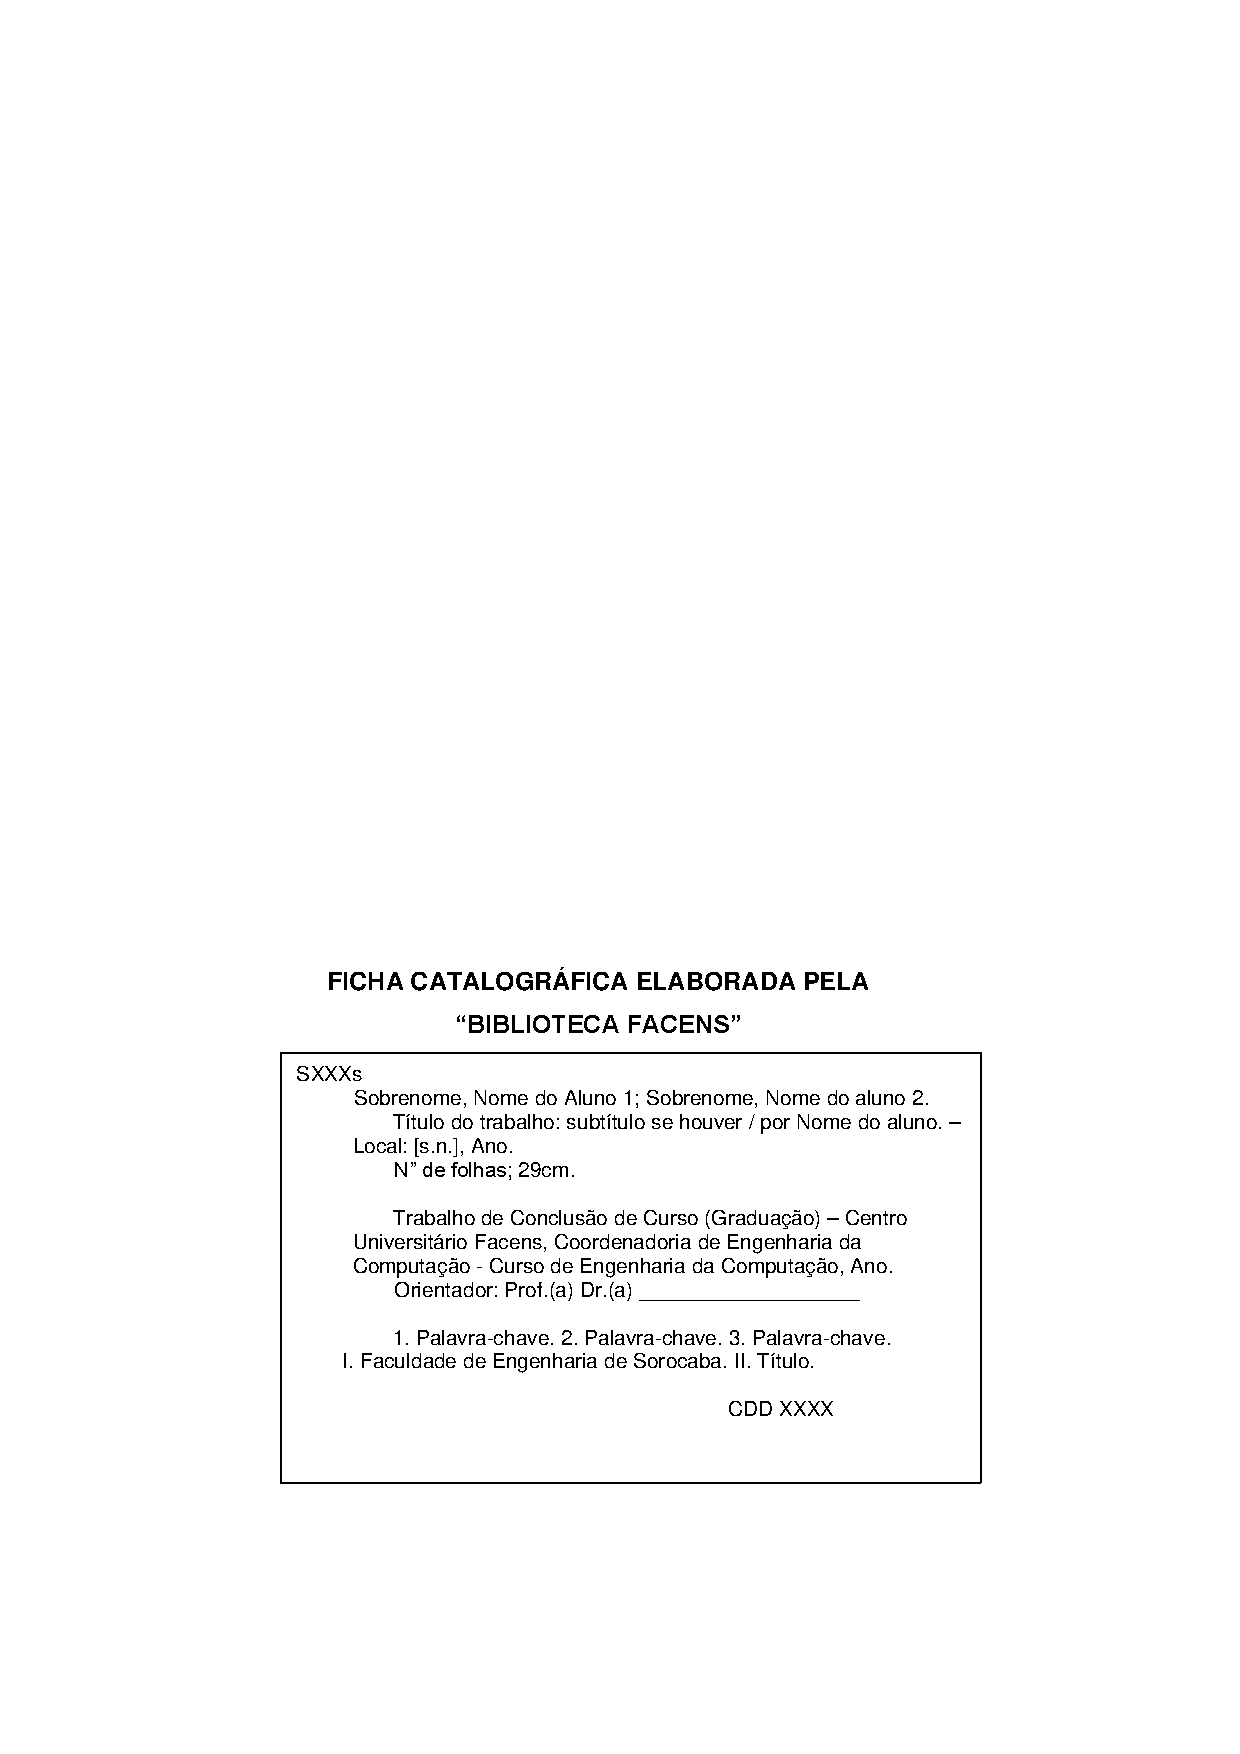
\includepdf[page=1]{partes/pre_textuais/ficha_catalografica.pdf}
\end{fichacatalografica}
\begin{folhadeaprovacao}

    \begin{center}
        {\ABNTEXchapterfont\large\imprimirautor}

        \vspace*{\fill}\vspace*{\fill}
        \begin{center}
            \ABNTEXchapterfont\bfseries\Large\imprimirtitulo
        \end{center}
        \vspace*{\fill}
        
        \hspace{.45\textwidth}
        \begin{minipage}{.5\textwidth}
            \imprimirpreambulo
        \end{minipage}%
        \vspace*{\fill}
    \end{center}
            
    Trabalho aprovado. \imprimirlocal, 24 de novembro de 2012:

    \assinatura{\textbf{\imprimirorientador} \\ Orientador} 
    \assinatura{\textbf{Professor} \\ Convidado 1}
    \assinatura{\textbf{Professor} \\ Convidado 2}
    %\assinatura{\textbf{Professor} \\ Convidado 3}
    %\assinatura{\textbf{Professor} \\ Convidado 4}
        
    \begin{center}
        \vspace*{0.5cm}
        {\large\imprimirlocal}
        \par
        {\large\imprimirdata}
        \vspace*{1cm}
    \end{center}
  
\end{folhadeaprovacao}
\begin{agradecimentos}
    Os agradecimentos principais são direcionados aos professores Andréia Lúcia Rodrigues, Johannes von Lochter, 
    Talita Berbel, Marco Antonio Montebello e demais professores da FACENS que contribuíram para a produção desta pesquisa acadêmica e 
    formação profissional de alta qualidade que a faculdade pôde oferecer.

    Agradecimentos especiais direcionados a familiares e amigos que de maneira direta e indireta fizeram a diferença na vida dos 
    membros desta pesquisa e com todos os méritos compartilham da conquista de sua realização.
    
    Por fim, agradecimentos direcionados a Fernando Haddad, Ministro da Educação 
    responsável pela criação do Programa Universidade para Todos, permitindo que os integrantes do 
    projeto pudessem ingressar e concluir a graduação sem custos.
\end{agradecimentos}
\begin{epigrafe}
    \vspace*{\fill}
	\begin{flushright}
        \textit{``Não vos amoldeis às estruturas deste mundo, \\
        mas transformai-vos pela renovação da mente, \\
        a fim de distinguir qual é a vontade de Deus: \\
        o que é bom, o que Lhe é agradável, o que é perfeito.\\
        (Bíblia Sagrada, Romanos 12, 2)}
	\end{flushright}
\end{epigrafe}
\setlength{\absparsep}{18pt} % ajusta o espaçamento dos parágrafos do resumo
\begin{resumo}
	Carros autônomos v{\^e}m sendo um campo de estudo cada vez mais discutido
	nos {\'u}ltimos anos, com um mercado em forte crescimento. Mesmo com
	esse crescimento, o mercado se v{\^e} restrito a poucas empresas, que
	est{\~a}o dispostas a arcar com os grandes investimento que o
	desenvolvimento e treinamento dessas solu{\c c}{\~o}es podem trazer. Com
	base nessa situa{\c c}{\~a}o, este projeto visa explorar uma alternativa ao
	modelo tradicional de carro aut{\^o}nomo, deixando de usar GPS e vis{\~a}o
	computacional e passando a se basear em aprendizado por refor{\c c}o, e
	principalmente no algoritmo NEAT (\textit{Neuroevolution of Augmenting
	Topologies}), um algoritmo baseado em redes neurais e algoritmo
	gen{\'e}tico para o aprendizado com m{\'i}nima necessidade de recursos —
	tanto em termos de aquisi{\c c}{\~a}o de dados quanto de performance. Foi
	criado um ambiente simulado em que o NEAT utiliza sensores de
	dist{\^a}ncia para progressivamente aprender a percorrer o caminho
	designado. Enquanto tenha sido obtido sucesso neste aprendizado, a
	inconsist{\^e}ncia na generaliza{\c c}{\~a}o da solu{\c c}{\~a}o encontrada
	pelo algoritmo (indicada pela performance na troca do percurso ap{\'o}s o
	treinamento) sugere a inaptid{\~a}o deste algoritmo a operar em ambientes
	imprevis{\'i}veis. Mesmo assim, a facilidade de treinamento e funcionamento
	fazem com que a utiliza{\c c}{\~a}o do NEAT seja sujeita a considera{\c
	c}{\~a}o em contextos de ambientes controlados e recursos limitados.

	\textbf{Palavras-chave}: Intelig{\^e}ncia Artificial. Aprendizado por Refor{\c c}o. Carros aut{\^o}nomos. Aprendizado de M{\'a}quina.
\end{resumo}

\begin{resumo}[Abstract]
	\begin{otherlanguage*}{english}
		Autonomous cars have been an increasingly discussed field of study in
		the last years, with a strong market growth. Even with this
		growth, the market is restricted to few companies that are willing to
		bear the great investments that the development and trainings of these
		solutions can bring. Based on this, this projects seeks to explore an
		alternative to the traditional autonomous car model, exchanging the use
		of GPS and computer vision with having a base on reinforcement
		learning, and primarily in the algorithm NEAT (\textit{Neuroevolution
		of Augmenting Topologies}), an algorithm based on neural networks and
		genetic algorithm for learning with minimum resources needed — both in
		monetary terms and in performance terms. A simulated environment was
		used in which NEAT uses distance sensors to progressively learn to
		travel the designaded path. While success was achieved in this
		training, the inconsistence of the generalization in the solution found
		by the algorithm (indicated by the performance when the track is
		switched after the training) suggests the inaptitude of the algorithm
		when operating in unpredictable environments. Nevertheless, the ease of
		training and operation make NEAT worth consideration in more
		predictable and low-resource contexts.

        \vspace{\onelineskip}

        \noindent 
        \textbf{Keywords}: Artificial Intelligence. Reinforcement Learning. Autonomous Cars. Machine Learning.
    \end{otherlanguage*}
\end{resumo}

\pdfbookmark[0]{\listfigurename}{lof}
\listoffigures*
\cleardoublepage
\pdfbookmark[0]{\listofquadrosname}{loq}
\listofquadros*
\cleardoublepage
\pdfbookmark[0]{\listtablename}{lot}
\listoftables*
\cleardoublepage
\begin{siglas}
    \item[ABNT] Associação Brasileira de Normas Técnicas
    \item[abnTeX] ABsurdas Normas para TeX
\end{siglas}
\pdfbookmark[0]{\contentsname}{toc}
\tableofcontents*
\cleardoublepage

% ----------------------------------------------------------
% ELEMENTOS TEXTUAIS
% ----------------------------------------------------------
\chapter{Introdução}
% ----------------------------------------------------------

De forma geral, esta monografia visa apresentar a implementação de um
ambiente simulado capaz de treinar um veículo autônomo que, através dos
casos de teste, consegue se adaptar ao ambiente em que se situa buscando
chegar a determinado objetivo, através de um algoritmo de neuroevolução que
possui uma topologia aumentante. Desta forma, simulações de possíveis trajetos
e adaptações de percurso podem ser rapidamente criadas e testadas sem a
necessidade de interação com um ambiente físico.

Tratando-se de veículos autônomos, é possível citar os carros sem
motorista, segundo \citeonline{arruda2015}, são veículos capazes de realizar tarefas
[...] sem a intervenção de operadores humanos, sua demanda vem crescendo
ultimamente por conta da acessibilidade que fornecem e por permitirem uma
produtividade maior ao motorista. Considerados também veículos autônomos,
existem aqueles voltados para sistemas logísticos, onde, através de mínima
interação com operadores, salvo manutenções e reprogramações, são capazes
de realizar transporte de objetos por uma linha de produção.

A solução geralmente aplicada para carros autônomos se fundamenta no
princípio da visão computacional. Esta técnica se baseia em utilizar de câmeras
para a captura de imagens que virão a servir de entrada de dados, para que o
algoritmo de direção tome as devidas decisões quanto à melhor decisão a ser
tomada para aquela situação.

O problema desta técnica se encontra justamente na lentidão de colocar
os sistemas em prática, pois é necessário que se criem diversas situações de
teste com muitas variáveis aplicáveis, como iluminação ou resolução da foto, e
considerando que a aplicação é direcionada a carros que navegarão pelas ruas,
é necessário que estes testes sejam prolongados ainda mais para que se haja
uma garantia de segurança a todos ao redor do veículo.

Ao observar veículos autônomos dentro do ambiente fabril, é possível
encontrar máquinas chamadas de Veículos Automaticamente Guiados (AGVs),
seu uso para o transporte de contêineres data de 1993 em um terminal de
contêineres de Rotterdan \cite{saputra2021}. Estes possuem a finalidade
de transportar materiais e produtos pela fábrica, através de sensores, são
capazes de identificar a distância necessária para a movimentação do garfo
quando aplicados a uma empilhadeira ou a distância de segurança para evitar
acidentes. A sua trajetória desses veículos é geralmente predefinida, baseando-
se na planta da fábrica e o caminho que o veículo deve percorrer, como através
de faixas magnéticas, por exemplo. Sendo assim, estes dispositivos falham
quando encontram obstáculos em seu caminho, como um pallet ou caixa que
manterão sua movimentação impedida.

Tratando-se de aprendizado de máquina, existem diversas técnicas que
podem ser empregadas para se chegar a resultados simulados, estas, focadas
na modelagem da estrutura de aprendizado podem ser divididas entre,
supervisionado, não supervisionado e por reforço. A aplicação de cada método
deve ser indicada de acordo com a necessidade da aplicação, e, analisando a
proposta do projeto presente nesta monografia, é possível analisar qual solução
possui a aplicação mais justificável. Em uma observação imediata, o
aprendizado por máquina supervisionado (aquele em que se sabe quais são as
possíveis entradas e saídas equivalentes a elas) se torna inviável, tal que a
aplicação exige que o algoritmo calcule em tempo real a intermissão de possíveis
objetos em seu trajeto, sendo assim impossível definir uma saída previamente.

Este projeto procura explorar um tipo diferente de aprendizado, chamado
de aprendizado por reforço. Esse tipo de aprendizado tem a característica de
não necessitar de supervisão para o treinamento do modelo. Ou seja, não se faz
necessário treinamento em campo ou uma requisição de grande quantidade de
dados para a etapa de treinamento. Como entradas para o modelo serão
utilizados sensores de distância, em vez dos habituais sistemas de visão
computacional. O experimento será feito dentro de um ambiente virtual, com a
representação do carro e trajetos gerados aleatoriamente para treinamento.

O método de aprendizado por reforço faz necessário menos investimentos
antecipados, pois os dados de treinamento serão obtidos por um quociente de
performance ao invés de dados rotulados para retroalimentação. Além disso, a
utilização de sensores diminui significativamente o requerimento de poder
computacional para o sistema comparado com processamento de imagens, e o
mesmo pode ser dito quanto ao algoritmo de aprendizado na etapa de testes.

O aprendizado se dará pelo algoritmo NEAT (Neuroevolution of
Augmenting Topologies). Este algoritmo se inicia com uma rede neural com
apenas as entradas e saídas definidas. Por meio de um Algoritmo Genético, o
algoritmo evoluirá a topologia da rede neural de forma a melhorar o desempenho
do carro (neste caso, conseguir dirigir por mais tempo sem colisões).

Por exemplo, a princípio o algoritmo gera diversos carros com topologias
aleatórias da rede neural. Os carros que percorrerem a maior distância sem
colisões serão selecionados para reprodução - seus genes serão combinados
com outros carros de performance alta, além de também ocorrerem mutações
para o descobrimento de novos comportamentos. Este processo criará uma nova
geração de carros, que passará pelos mesmos testes, e o processo se repetirá.

Deste modo, espera-se atingir um estado de otimização em que se faz
possível o alcance da trajetória especificada sem colisões, e preferivelmente em
um caminho próximo do mais otimizado.

Apesar da elevada facilidade introduzida com esse método, a perda de
flexibilidade na utilização pode ser algo que geraria necessidade de um sistema
mais robusto como o de visão computacional. Um outro contraponto seria a
necessidade de um ambiente mais controlado, para certificar um funcionamento
correto dos sensores no ambiente e nos possíveis obstáculos. Mesmo com tais
observações, existe margem para crer que o método proposto se faz uma
alternativa interessante em aplicações em que as condições de funcionamento
podem ser mapeadas previamente.

\include{abntex2-modelo-include-comandos}

\chapter{Referencial teórico}\label{cap_trabalho_academico}

\section{Aliquam vestibulum fringilla lorem}

\lipsum[1]

\lipsum[2-3]
\chapter{Metodologias}

\lipsum[1]

\section{Simula{\c c}{\~a}o}

\lipsum[2-3]

\section{Implementa{\c c}{\~a}o}

\lipsum[4-6]

\section{Treinamento}

\lipsum[7-8]


\chapter{Resultados}

O problema proposto, o qual os testes serão realizados, se dá no próprio
ambiente de simulação de carros autônomos criado previamente. Com o objetivo de
medir o impacto do diferencial do NEAT - suas topologias aumentantes - serão
aplicados tr{\^e}s diferentes m{\'e}todos de treinamento:

\begin{enumerate}
	\item NEAT, proveniente do \textit{neat-python} pós parametrização, com topologia inicial m{\'i}nima;
	\item Neuroevolução, através da aplicação de um algoritmo genético sobre uma rede neural simples (sem topologias aumentantes);
	\item NEAT, com topologia inicial complexa.
\end{enumerate}

%% FIXME: generalidade?
Alem desses, ser{\'a} tamb{\'e}m aplicado um teste de adapta{\c c}{\~a}o no
algoritmo, trocando a pista apos o seu treinamento com fim de medir a
generalidade da tomada de decis{\~a}o.

Tais algoritmos trabalham de diferentes formas a encontrar valores de aptidão
para suas simulações. De modo a generalizar a classificação de resultados, foi
proposto a construção de um valor de pontua{\c c}{\~a}o atrelado à distância percorrida pelo
carro em sua execução.

Esta métrica pode vir a ser comparada entre métodos a fim de se encontrar
quanto tempo é necessário para se alcançar determinada fitness e quanto é
alcançado após determinado tempo de execução decorrer.

Os resultados foram obtidos de duas diferentes formas: primeiramente
encontrando em que geração do algoritmo este consegue alcançar um valor de
\textit{fitness} mínimo necessário para que o carro execute uma volta completa pelo
trajeto, definindo assim quão rapidamente ele consegue alcançar uma resposta. A
\autoref{fig_meta} ilustra dentro do ambiente de simulação o alvo a ser alcançado.

\begin{figure}[htb]
        \centering
        \caption{\label{fig_meta}Canto inferior esquerdo definido como meta a ser alcançada para obtenção de resultado.}
        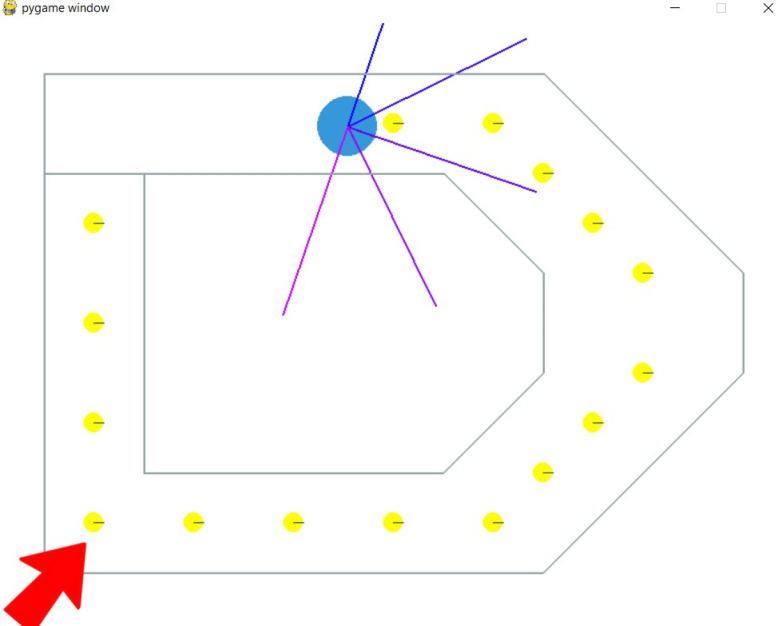
\includegraphics[width=0.5\textwidth]{images/meta.png}
        \legend{
                Fonte: Autoria Pr{\'o}pria.
        }
\end{figure}

A Rede Neural inicial é composta por 5 sensores que verificam e alimentam a
rede a cada movimento do carro e são elencados com os valores que vão de -5 até
-1. Essas 5 entradas estão todas conectadas a cada um das 3 saídas que indicam
a direção que o carro deve tomar, as saídas vão de 0 até 2, sendo 0 a indicação
de movimento a esquerda, 1 a direito e 2 para frente. Cada conexão entre cada
sensor de entrada e cada nó de saída possui um peso específico que serve para a
geração do valor de saída. A estrutura indicada acima pode ser encontrada na
\autoref{fig_nn1} abaixo.

\begin{figure}[htb]
        \centering
        \caption{\label{fig_nn1}Organização da rede, com seus nós e conexões.}
        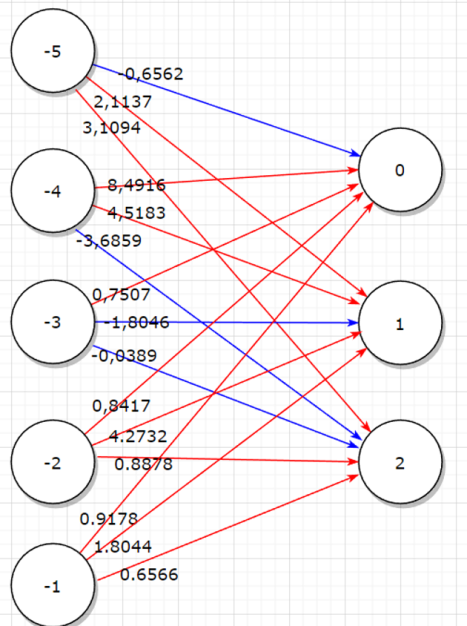
\includegraphics[width=0.4\textwidth]{images/nn1.png}
        \legend{
                Fonte: Autoria Pr{\'o}pria.
        }
\end{figure}

O processo de aprendizado de uma determinada rede veio a ser executado em um
ambiente de treinos, o qual, tratando-se do algoritmo NEAT, a topologia parte
de seu estado mais simples até possuir um determinado formato da qual é capaz
de finalizar o percurso, sendo tratada como a resposta ideal proposta. O
algoritmo de Neuroevolução também parte de seu estado mais simples até as
respostas desejadas neste ambiente.

\section{NEAT}

A simulação do treino para o algoritmo NEAT incorpora o aumento das topologias,
este pode vir a ser dado pela possibilidade de adições e subtrações de nós nas
camadas ocultas da rede e/ou remoção ou adição de conexões entre nós, fatores
observados nas redes dos resultados alcançados.

Foram realizadas três execuções com o objetivo de se alcançar a fitness mínima
para que uma volta completa seja realizada em torno da pista, mensurado como
cerca de 16000 pontos de aptidão com 300 membros na população. Os resultados
com as respectivas gerações em que o cálculo foi alcançado se dão na \autoref{tabela_neat},
juntamente da topologia resultante em cada iteração.

\begin{table}[htb]
	\centering
    \caption{\label{tabela_neat}Resultados obtidos pelo NEAT até a meta de Fitness ser alcançada.}
    \begin{tabular}{ccccc}
        \hline
		\textbf{Itera{\c c}{\~o}es} & \textbf{Topologia} & \textbf{Gera{\c c}{\~a}o} & \textbf{\textit{Fitness}} & \textbf{\textit{Fitness} média} \\ \hline
		1 & (3,13)  & 8   & 16379  & 3664 ± 2106   \\ \hline
		2 & (3,14)  & 3   & 16337  & 3285 ± 2165   \\ \hline
		3 & (4,13)  & 8   & 16336  & 3684 ± 2126   \\ \hline
    \end{tabular}
    \fonte{Autoria pr{\'o}pria.}
\end{table}

Como observável na \autoref{fig_nn2}, a terceira iteração obteve uma  topologia
a qual indica a existência de quatro nós e treze conexões totais, este nó
intermediário, inserido após um processo de mutação, serve como uma conexão na
camada oculta entre a entrada -2 e as saídas 1 e 2. Além desta alteração, a
topologia também sofreu alterações com a remoção da conexão entre a entrada -3
e saída 0, julgada pelo algoritmo como uma melhoria para o desempenho durante
suas mutações e cruzamentos.

\begin{figure}[htb]
        \centering
        \caption{\label{fig_nn2}Rede neural da Iteração 3 de treinos do algoritmo NEAT, com uma conexão excluída e um nó adicional na camada oculta.}
        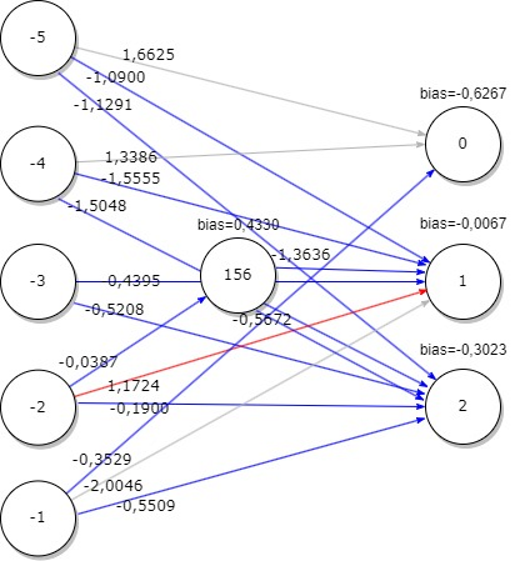
\includegraphics[width=0.4\textwidth]{images/nn2.png}
        \legend{
                Fonte: Autoria Pr{\'o}pria.
        }
\end{figure}

A segunda bateria de treinos englobava a execução do algoritmo até sua 10ª
geração, e a comparação dos resultados obtidos até então. Seus resultados são
observáveis na \autoref{tabela_neat_10}.

\begin{table}[htb]
	\centering
    \caption{\label{tabela_neat_10}Resultados obtidos pelo NEAT após a execução de 10 gerações.}
    \begin{tabular}{ccccc}
        \hline
		\textbf{Itera{\c c}{\~o}es} & \textbf{Topologia} & \textbf{Gera{\c c}{\~a}o} & \textbf{\textit{Fitness}} & \textbf{\textit{Fitness} média} \\ \hline
		1 & (4,9)   & 10  & 16383  & 3191 ± 2524   \\ \hline
		2 & (3,12)  & 10  & 18528  & 3847 ± 1997   \\ \hline
		3 & (4,15)  & 10  & 14199  & 3569 ± 1903   \\ \hline
    \end{tabular}
    \fonte{Autoria pr{\'o}pria.}
\end{table}

Observando a topologia da iteração de número 2, é possível verificar que esta
que obteve a maior \textit{fitness} em 10 gera{\c c}{\~o}es, identificou como
uma melhora no resultado a quebra da conexão entre a entrada -5 e a saída 0 e a
entrada -1 e saída 2, como observável na \autoref{fig_nn3}.

\begin{figure}[htb]
        \centering
        \caption{\label{fig_nn3}Rede neural da Iteração 2 de treinos do algoritmo NEAT, com duas conexões excluídas e uma desativada.}
        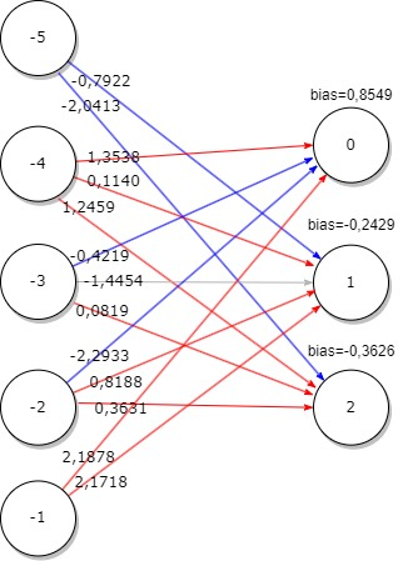
\includegraphics[width=0.4\textwidth]{images/nn3.png}
        \legend{
                Fonte: Autoria Pr{\'o}pria.
        }
\end{figure}

\section{Neuroevolu{\c c}{\~a}o}

Para a simulação de um algoritmo básico de Neuroevolução sem a etapa de aumento
de topologias, se fez uso da mesma estrutura utilizada anteriormente pelo NEAT,
porém sem a possibilidade de haver adições ou subtrações de nós (nas camadas
ocultas) ou conexões (entre entradas, nós e saídas).

Como apresentado na \autoref{tabela_ne}, o algoritmo foi executado três vezes com
diferentes valores para \textit{fitness} alcançada e em que geração esta se deu,
considerando uma população de 300 integrantes.

A coluna de topologia não se faz necessária considerando que este, por se
tratar de um algoritmo simples de neuroevolução, possui suas tomadas de
decisões realizadas apenas na pesagem de suas arestas, sem alterações de
topologia durante a execução.

\begin{table}[htb]
	\centering
    \caption{\label{tabela_ne}Resultados obtidos em suas respectivas gerações após execução do algoritmo de Neuroevolução.}
    \begin{tabular}{cccc}
        \hline
		\textbf{Itera{\c c}{\~o}es} & \textbf{Gera{\c c}{\~a}o} & \textbf{\textit{Fitness}} & \textbf{\textit{Fitness} média} \\ \hline
		1 & 3   & 16345  & 3354 ± 2138   \\ \hline
		2 & 12  & 16373  & 3839 ± 1930   \\ \hline
		3 & 12  & 16382  & 3788 ± 2298   \\ \hline
    \end{tabular}
    \fonte{Autoria pr{\'o}pria.}
\end{table}

A rede neural referente à iteração que alcançou o resultado mais rapidamente
pode ser expressa na \autoref{fig_nn4}, com suas devidas conexões e pesos.

\begin{figure}[htb]
        \centering
        \caption{\label{fig_nn4}Rede neural da Iteração 1 de treinos do algoritmo de Neuroevolução.}
        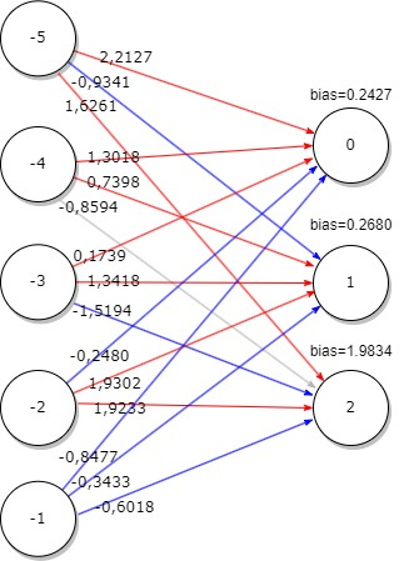
\includegraphics[width=0.4\textwidth]{images/nn4.png}
        \legend{
                Fonte: Autoria Pr{\'o}pria.
        }
\end{figure}

A \autoref{tabela_ne_10} ilustra os resultados obtidos para o algoritmo de
Neuroevolução considerando três execuções até a décima geração, com a fitness
média e máxima alcançadas dentro da população de 300 integrantes para cada
iteração. Do mesmo modo, a rede neural com o resultado da iteração de melhor
resultado pode ser expressa na \autoref{fig_nn5}, com suas devidas conexões e
pesos.

\begin{table}[htb]
	\centering
    \caption{\label{tabela_ne_10}Resultados obtidos até a décima geração após execução do algoritmo de Neuroevolução.}
    \begin{tabular}{cccc}
        \hline
		\textbf{Itera{\c c}{\~o}es} & \textbf{Gera{\c c}{\~a}o} & \textbf{\textit{Fitness}} & \textbf{\textit{Fitness} média} \\ \hline
		1 & 10  & 16356  & 3754 ± 2159   \\ \hline
		2 & 10  & 19596  & 3923 ± 2101   \\ \hline
		3 & 10  & 16335  & 3767 ± 1966   \\ \hline
    \end{tabular}
    \fonte{Autoria pr{\'o}pria.}
\end{table}

\begin{figure}[htb]
        \centering
        \caption{\label{fig_nn5}Rede neural da Iteração 2 após 10 gerações de treinos do algoritmo de Neuroevolução.}
        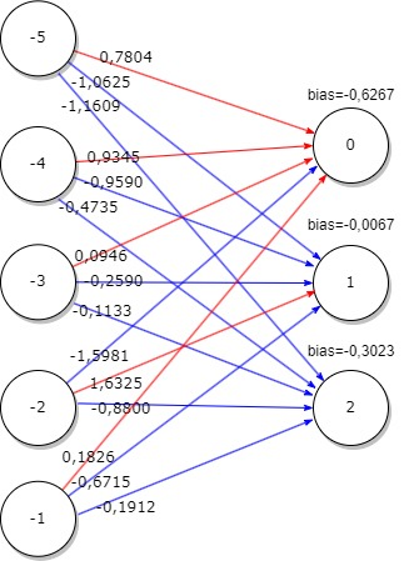
\includegraphics[width=0.4\textwidth]{images/nn5.png}
        \legend{
                Fonte: Autoria Pr{\'o}pria.
        }
\end{figure}

\section{NEAT com Topologia Inicial Complexa}

\begin{table}[htb]
	\centering
    \caption{\label{tabela_neatc}Resultados obtidos pelo NEAT com topologia inicial complexa até a meta de Fitness ser alcançada.}
    \begin{tabular}{ccccc}
        \hline
		\textbf{Itera{\c c}{\~o}es} & \textbf{Topologia} & \textbf{Gera{\c c}{\~a}o} & \textbf{\textit{Fitness}} & \textbf{\textit{Fitness} média} \\ \hline
		1 & (8,40)  & 23  & 16339  & 1010 ± 2314   \\ \hline
		2 & (8,39)  & 2   & 16429  & 1220 ± 1992   \\ \hline
		3 & (8,39)  & 23  & 16319  & 1379 ± 2785   \\ \hline
    \end{tabular}
    \fonte{Autoria pr{\'o}pria.}
\end{table}

Pode-se observar a elevada vari{\^a}ncia dos resultados - indicando uma
dificuldade do algoritmo evitar os m{\'a}ximos locais com essa quantidade
elevada de n{\'o}s. Outro ponto seria o mantenimento da topologia - o algoritmo
teve melhor performance ao evitar a remo{\c c}{\~a}o de nodes, e removendo
somente uma ou at{\'e} nenhuma das conex{\~o}es.

Tamb{\'e}m percebe-se a occor{\'e}ncia m{\'u}ltipla da gera{\c c}{\~a}o 32 -
isso se d{\'a} pelo funcionamento interno do \textit{neat-python}, em que a
partir da gera{\c c}{\~a}o 20 come{\c c}a a eliminar as esp{\'e}cies
\textit{estagnadas}, ou seja, indiv{\'i}duos que estavam sendo utilizados pela
possibilidade de haver caracter{\'i}sticas {\'u}teis, por{\'e}m n{\~a} deram
resultado. Com essa popula{\c c}{\~a}o removida, o algoritmo consegue assim
atingir o objetivo em algumas gera{\c c}{\~o}es.

\section{Adapta{\c c}{\~a}o a ambiente de testes}

%% FIXME: generalidade?
O ambiente de teste foi estruturado como mostrado na \autoref{fig_teste}, de
modo semelhante ao ambiente de treino por{\'e}m com altera{\c c}{\~o}es no
percurso de modo a testar a generalidade da solu{\c c}{\~a}o encontrada. Os
algoritmos foram rodados at{\'e} a meta previamente determinada (em torno de
16000 de \textit{fitness}) e no fim do treinamento foram expostos ao novo
ambiente, tendo a medida de sua dist{\^a}ncia percorrida at{\'e} a primeira
colis{\~a}o.

\begin{figure}[htb]
        \centering
        \caption{\label{fig_teste}Percurso alternativo de teste.}
        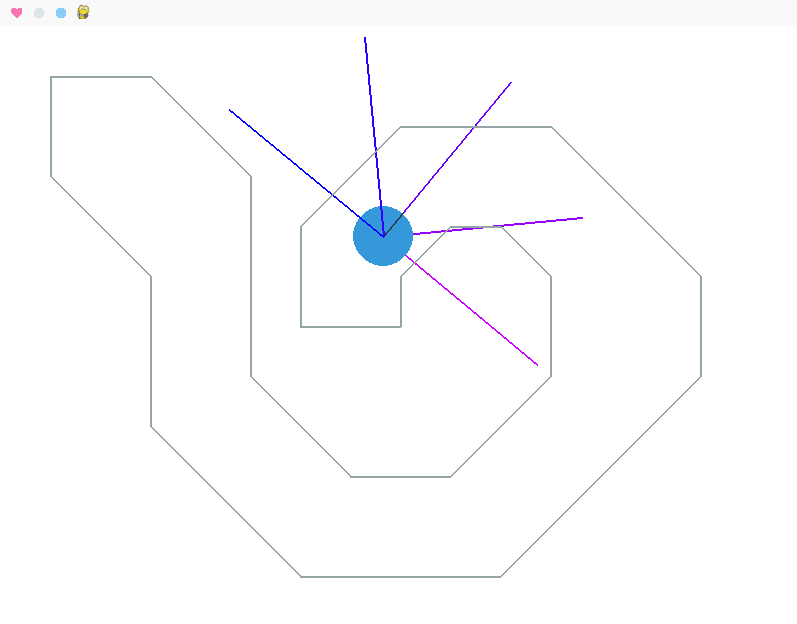
\includegraphics[width=0.5\textwidth]{images/teste.png}
        \legend{
                Fonte: Autoria Pr{\'o}pria.
        }
\end{figure}

Uma medida de sucesso seria o percorrimento do caminho completo, o que foi
medido como sendo um numero proximo de 1200 de dist{\^a}ncia.

Aplicando essa t{\'e}cnica com o algoritmo NEAT parametrizado, se obteve os
resultados apresentados na \autoref{tabela_teste_neat}.

\begin{table}[htb]
	\centering
	\caption{\label{tabela_teste_neat}Resultados obtidos pelo NEAT sendo exposto a um ambiente diferente ap{\'o}s a meta de Fitness ser alcançada.}
    \begin{tabular}{ccccc}
        \hline
		\textbf{Itera{\c c}{\~o}es} & \textbf{Topologia} & \textbf{Gera{\c c}{\~a}o} & \textbf{\textit{Fitness}} & \textbf{Resultado do teste} \\ \hline
		1 & (3,13)  & 9   & 16384  & 1386   \\ \hline
		2 & (4,12)  & 8   & 16412  & 134    \\ \hline
		3 & (3,12)  & 7   & 16348  & 250    \\ \hline
    \end{tabular}
    \fonte{Autoria pr{\'o}pria.}
\end{table}

Aplicando o mesmo para a neuroevolu{\c c}{\~a}o sem topologias vari{\'a}veis,
se obteve os resultados apresentados na \autoref{tabela_teste_ne}.

\begin{table}[htb]
	\centering
	\caption{\label{tabela_teste_ne}Resultados obtidos pela neuroevolu{\c c}{\~a}o sem topologia vari{\'a}vel sendo exposta a um ambiente diferente ap{\'o}s a meta de Fitness ser alcançada.}
    \begin{tabular}{ccccc}
        \hline
		\textbf{Itera{\c c}{\~o}es} & \textbf{Topologia} & \textbf{Gera{\c c}{\~a}o} & \textbf{\textit{Fitness}} & \textbf{Resultado do teste} \\ \hline
		1 & (3,15)  & 8   & 16357  & 167  \\ \hline
		2 & (3,15)  & 16  & 16354  & 16   \\ \hline
		3 & (3,15)  & 4   & 16319  & 22   \\ \hline
    \end{tabular}
    \fonte{Autoria pr{\'o}pria.}
\end{table}

Por fim aplicando o mesmo para o NEAT com topologia complexa inicial, se obteve
os resultados apresentados na \autoref{tabela_teste_neatc}.

\begin{table}[htb]
	\centering
	\caption{\label{tabela_teste_neatc}Resultados obtidos pelo NEAT com topologia inicial complexa sendo exposto a um ambiente diferente ap{\'o}s a meta de Fitness ser alcançada.}
    \begin{tabular}{ccccc}
        \hline
		\textbf{Itera{\c c}{\~o}es} & \textbf{Topologia} & \textbf{Gera{\c c}{\~a}o} & \textbf{\textit{Fitness}} & \textbf{Resultado do teste} \\ \hline
		1 & (8,39)  & 23  & 16390  & 1129   \\ \hline
		2 & (8,38)  & 22  & 16397  & 180   \\ \hline
		3 & (8,38)  & 2   & 16328  & 133   \\ \hline
    \end{tabular}
    \fonte{Autoria pr{\'o}pria.}
\end{table}

\section{Analise de resultados}

%% TODO: Finalizar

Parametrizacao normal com topologia chega a um resultado de fitness consideravelmente rapido mas acaba falhando no teste.

neuroevolucao simples ficou proxima do neat, demorando um pouco mais para atingir fitness maiores porem consistentemente ficando melhor a longo prazo.

Topologia inicial complexa mais sucessivel a maximo local, e evitou remover nodes - mesmo assim, a topologia elevada levou a solu{\c c}{\~o}es mais inteligentes

\chapter{Considerações finais}

\textbf{***Paralelizacao e desempenho vs deep q learning; predominancia de carros andando em circulo***}

\lipsum[31-33]


% ----------------------------------------------------------
% ELEMENTOS PÓS-TEXTUAIS
% ----------------------------------------------------------
\bibliography{abntex2-modelo-references}

\begin{apendicesenv}
    \chapter{Quisque libero justo}
    \lipsum[50]

    \chapter{Nullam elementum urna vel imperdiet sodales elit ipsum pharetra ligula
    ac pretium ante justo a nulla curabitur tristique arcu eu metus}
    \lipsum[55-57]
\end{apendicesenv}
\begin{anexosenv}
    \chapter{Morbi ultrices rutrum lorem.}
    \lipsum[30]

    \chapter{Cras non urna sed feugiat cum sociis natoque penatibus et magnis dis
    parturient montes nascetur ridiculus mus}
    \lipsum[31]

    \chapter{Fusce facilisis lacinia dui}
    \lipsum[32]
\end{anexosenv}

%---------------------------------------------------------------------
% INDICE REMISSIVO
%---------------------------------------------------------------------
\printindex
%---------------------------------------------------------------------

\end{document}
